\documentclass[xcolor=dvipsnames,aspectratio=1610]{beamer}

\usepackage{graphicx}
\usepackage[scale=2]{ccicons}

\usetheme[numbering=counter, progressbar=frametitle, sectionpage=none]{metropolis}
\setbeamercolor{background canvas}{bg=white}


\title{Conflict-Free Vertex Coloring of Planar Graphs}
\date{April 15, 2017}
\author{Shawn Seymour}

\begin{document}
  \maketitle

  \begin{frame}
    \begin{figure}[h]
      \centering
      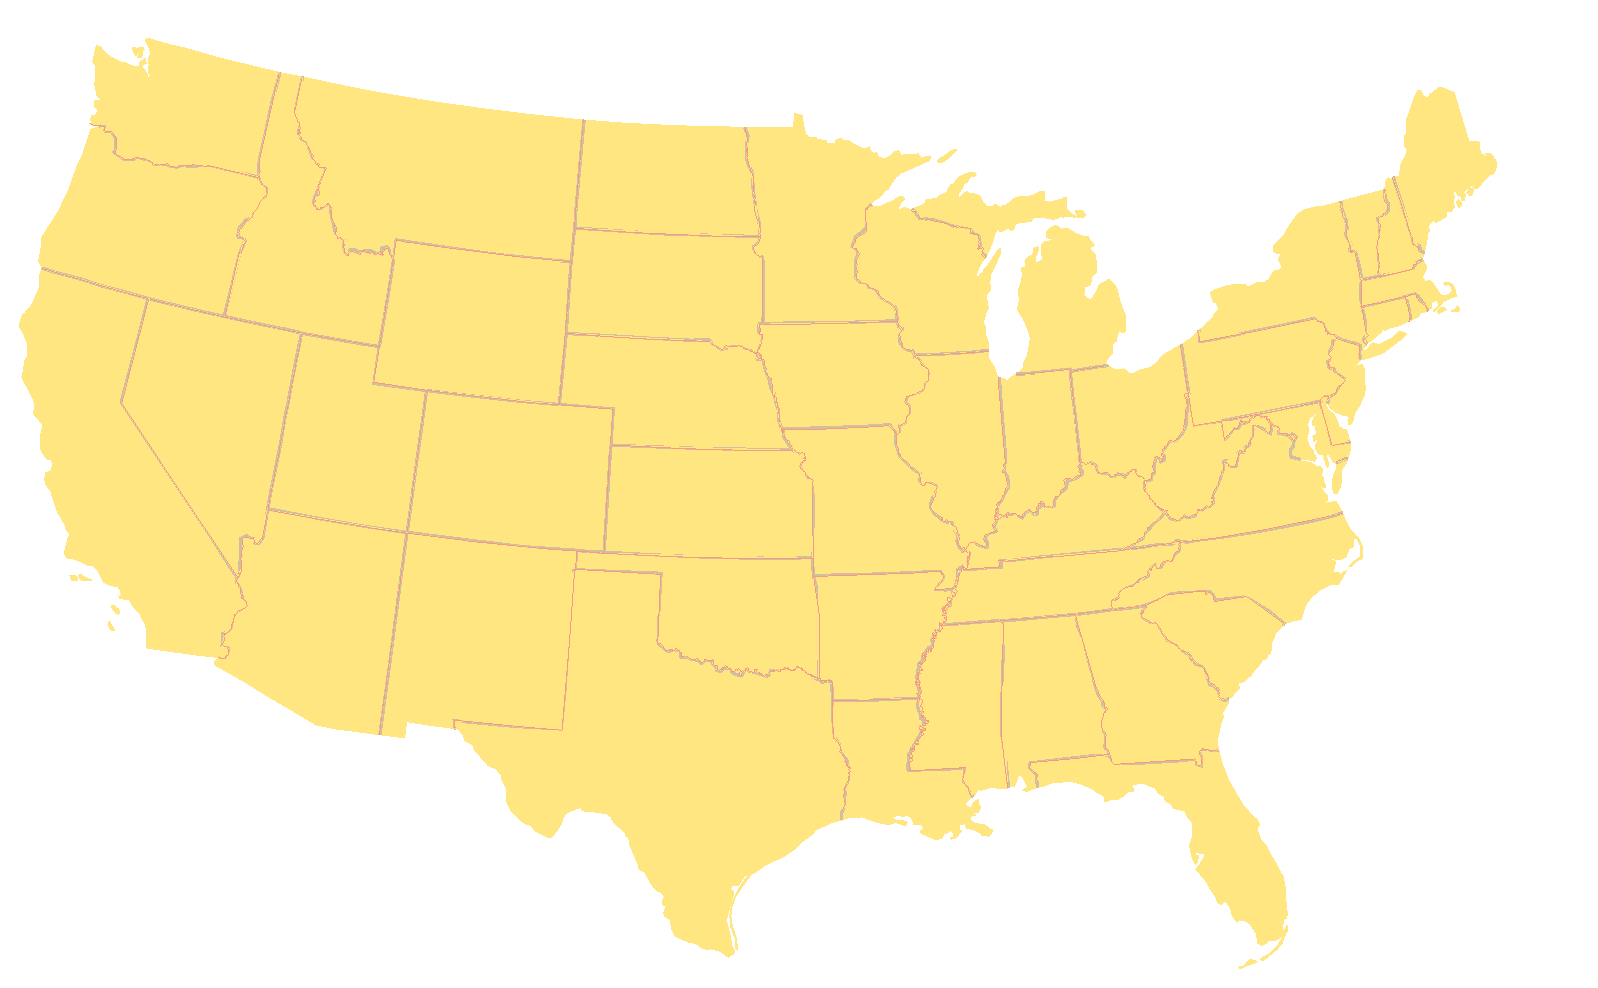
\includegraphics[width=14cm]{../figures/map-no-colors.pdf}
    \end{figure}
  \end{frame}

  \begin{frame}
    \begin{figure}[h]
      \centering
      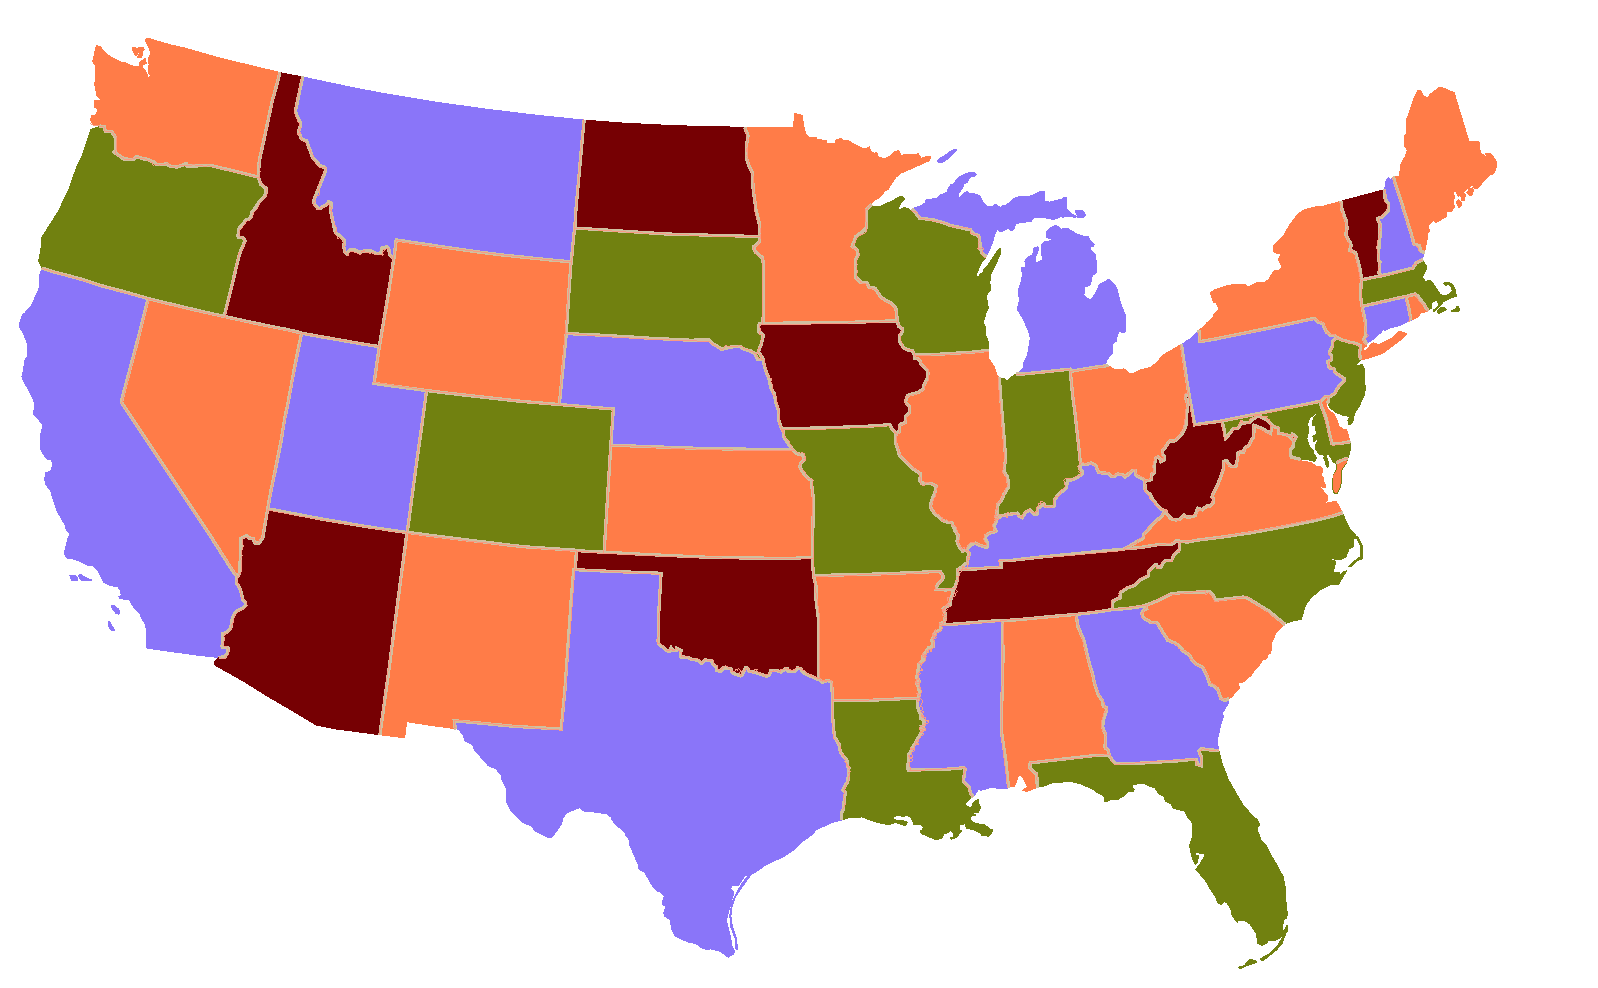
\includegraphics[width=14cm]{../figures/map-colors.pdf}
    \end{figure}
  \end{frame}

  \section*{Background}

  \subsection*{Graph Theory}

  \begin{frame}
    \frametitle{Graph Theory}

    \begin{figure}[h]
      \centering
      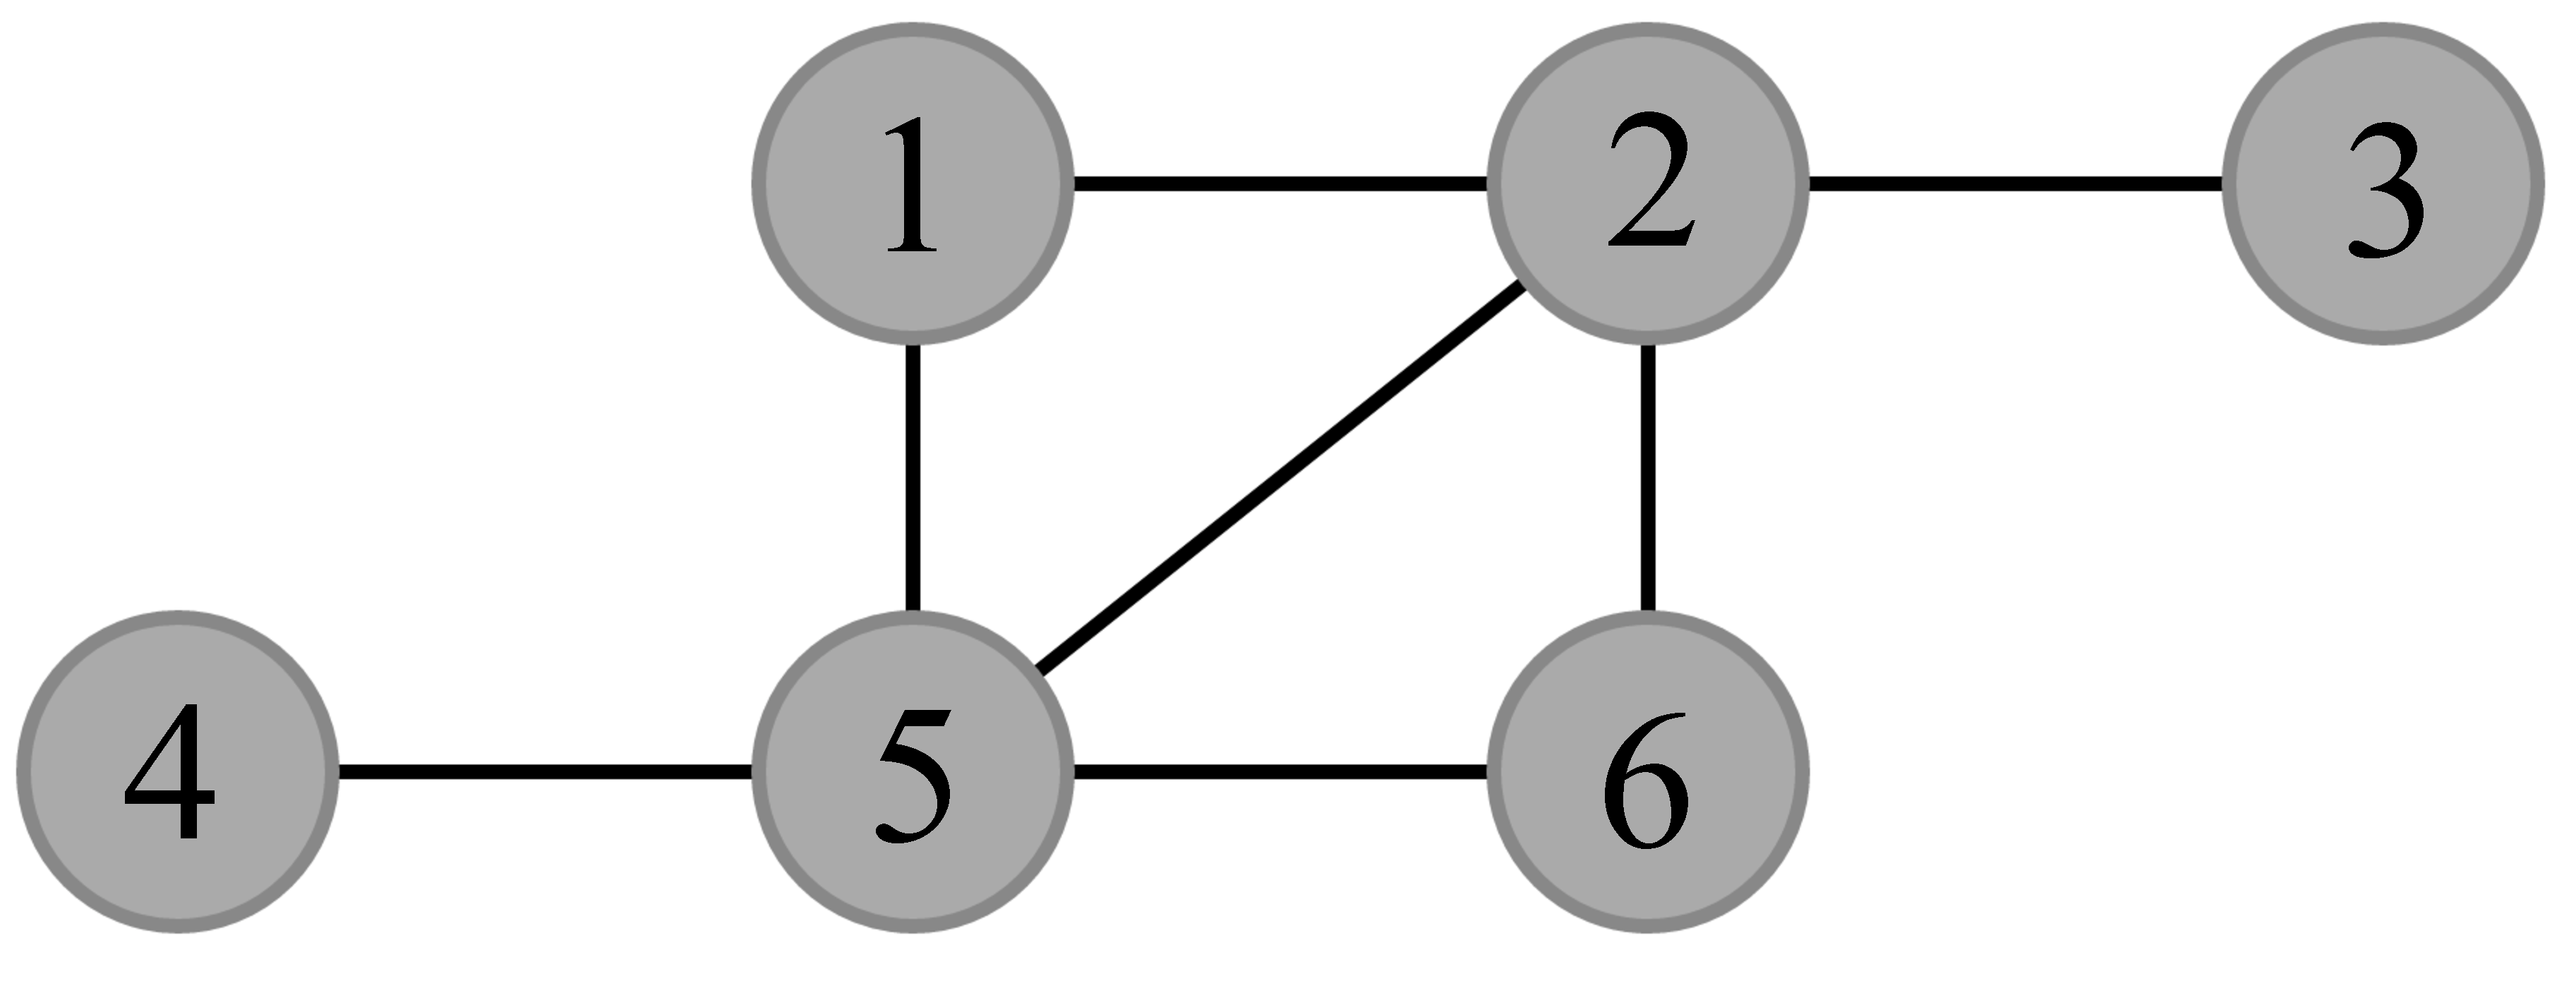
\includegraphics[width=8cm]{../figures/example.pdf}
    \end{figure}

    \vfill

    \begin{itemize}
      \item A \textbf{graph} is a set of vertices \emph{V} and a set of edges \emph{E}.
      \item The \textbf{neighborhood} of a vertex $v$ is a set of all vertices adjacent to $v$.
      \item The \textbf{closed neighborhood} of $v$ includes the neighborhood of $v$ and $v$ itself.
    \end{itemize}
  \end{frame}

  \subsection*{Graph Coloring}

  \begin{frame}
    \frametitle{Vertex Coloring}

    \begin{figure}[h]
      \centering
      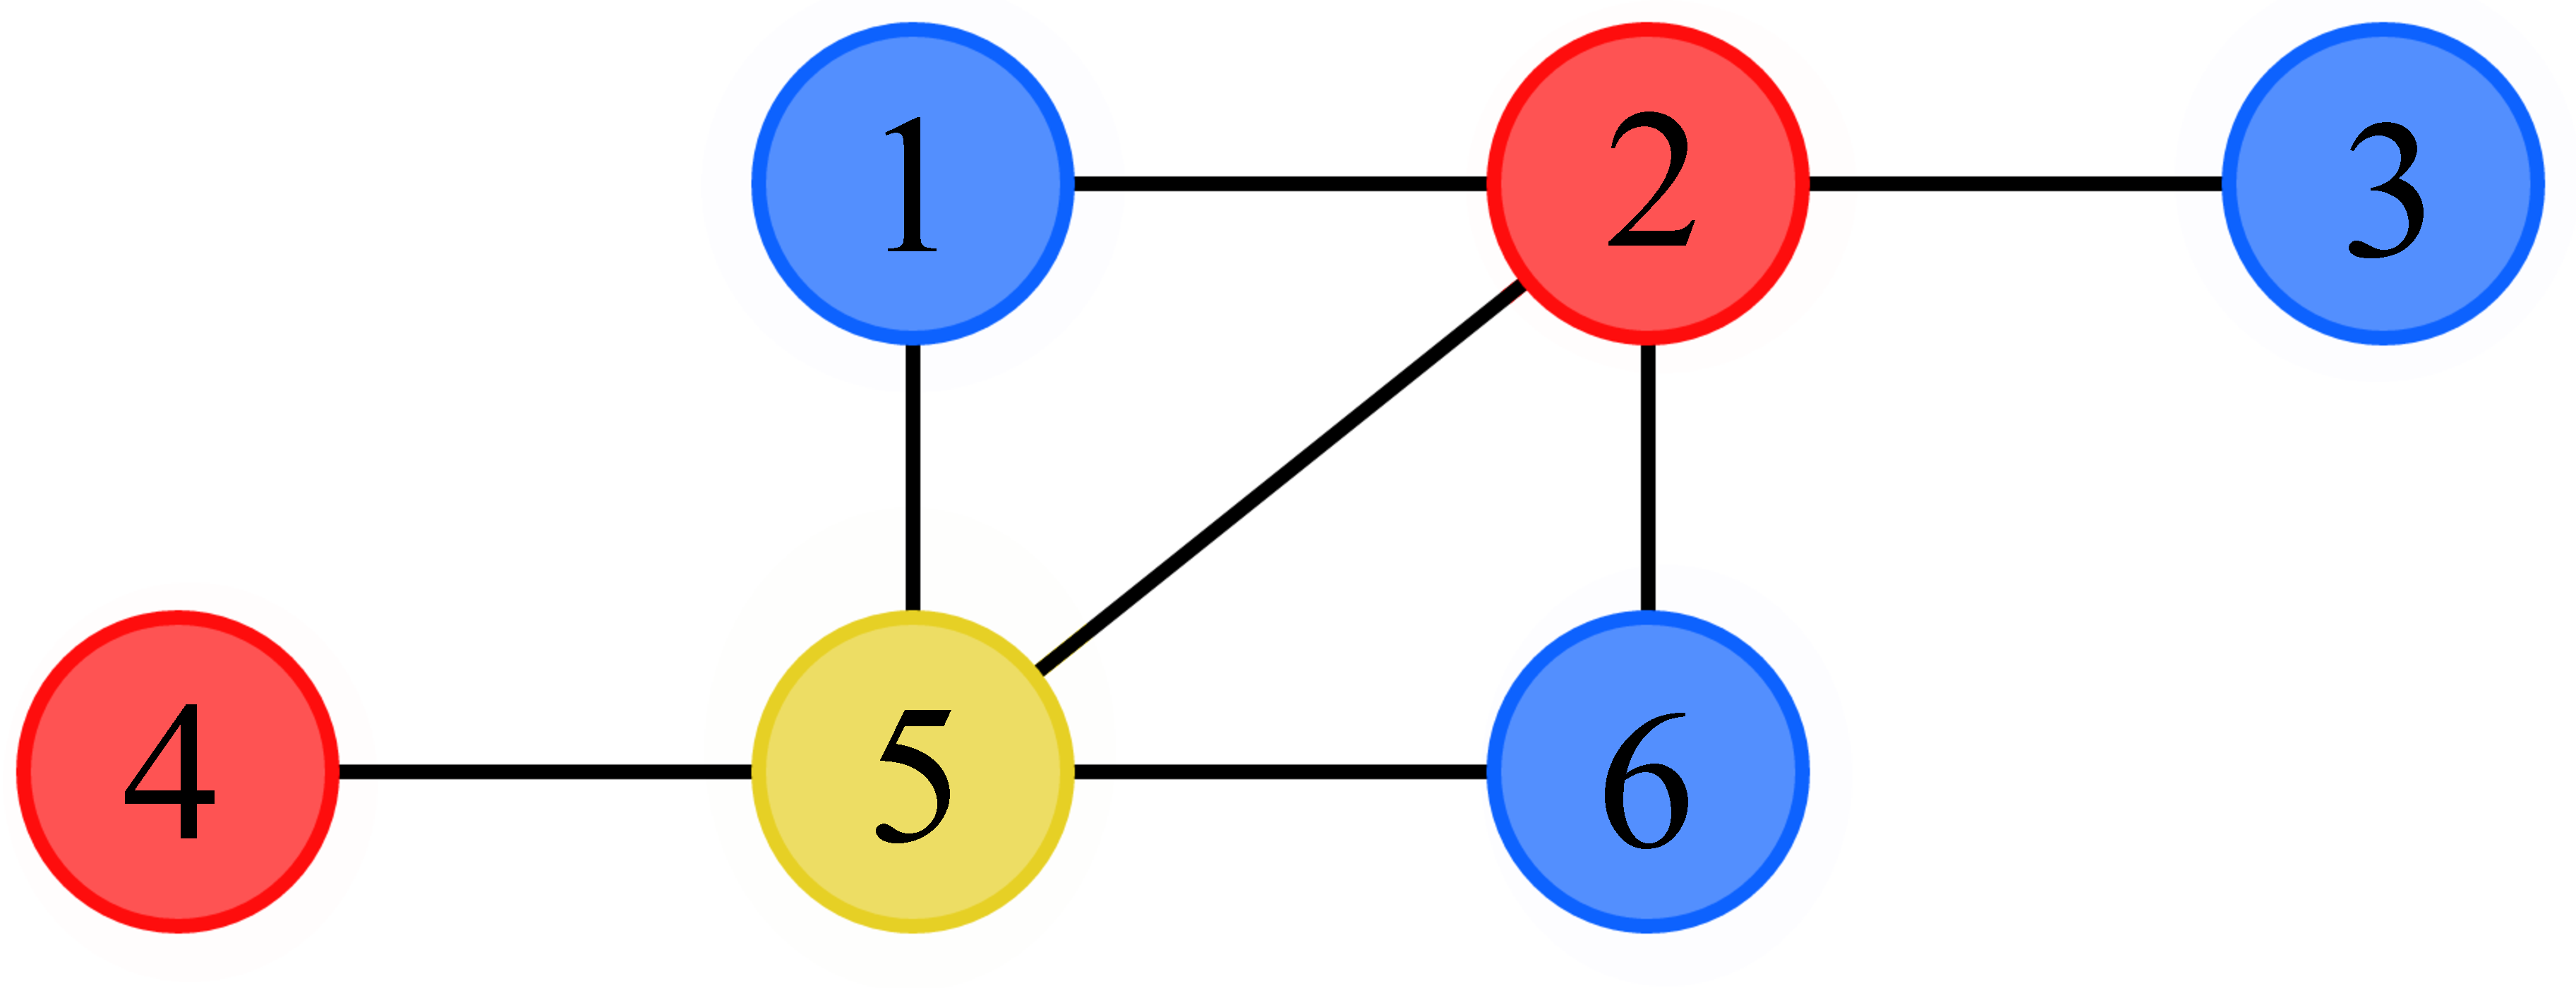
\includegraphics[width=8cm]{../figures/example-vcp.pdf}
    \end{figure}

    \vfill

    \begin{itemize}
      \item A proper \textbf{vertex coloring} of a graph $G$ is an assignment of colors to each vertex such that no adjacent vertices share the same color.
      \item The \textbf{chromatic number} of $G$ is the minimum number of colors needed to properly color $G$.
    \end{itemize}
  \end{frame}

  \begin{frame}
    \frametitle{Conflict-Free Coloring}

    \begin{figure}[h]
      \centering
      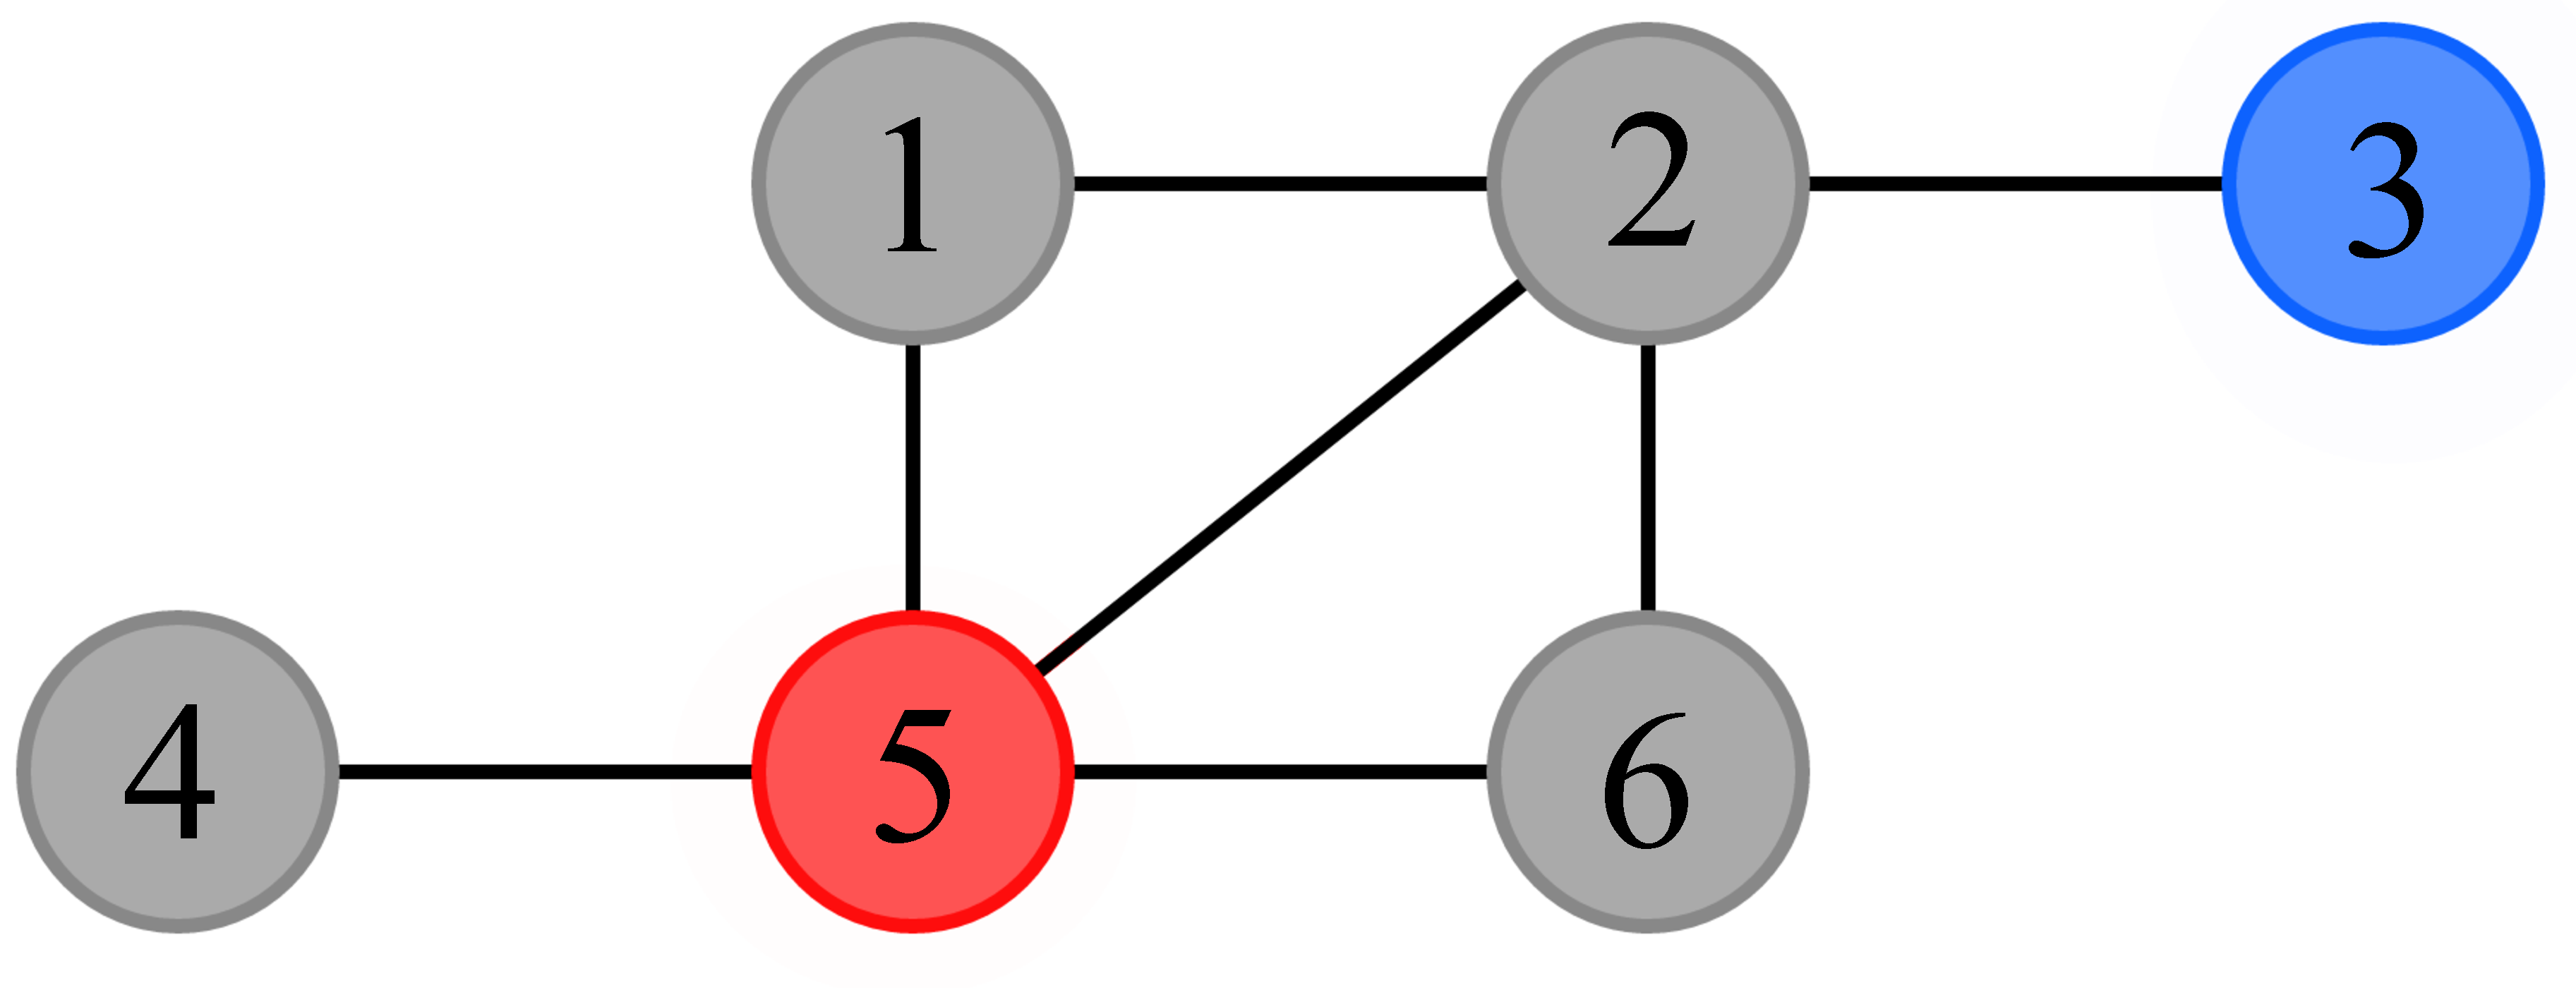
\includegraphics[width=8cm]{../figures/example-cfcp.pdf}
    \end{figure}

    \vfill

    \begin{itemize}
      \item A \textbf{conflict-free coloring} of a graph $G$ assigns one of $k$ colors to some of the vertices such that, for every vertex $v$, there is a unique color assigned to a vertex among $v$ and $v$'s neighbors.
      \item Every proper vertex coloring of $G$ is also a conflict-free coloring of $G$. This is because every vertex can be its own conflict-free neighbor.
    \end{itemize}
  \end{frame}

  \begin{frame}[standout]
    \centering
    Thanks to Peter Dolan and Elena Machkasova for their advice and feedback.
    \vfill
    \href{https://github.com/devshawn/senior-seminar}{github.com/devshawn/senior-seminar}
    \vfill
    \ccbyncsa{}
  \end{frame}

\end{document}
